
The majority of this book will teach you how to prepare CMake projects for your users. To cater to their needs, we need to thoroughly understand how users interact with CMake in different scenarios. This will allow you to test your project files and ensure they're working correctly.

CMake is a family of tools and consists of five executables:

\begin{itemize}
\item 
cmake: This is the main executable that configures, generates, and builds projects.

\item 
ctest: This is the test driver program used to run and report test results.

\item 
cpack: This is the packaging program used to generate installers and source packages.

\item 
cmake-gui: This is the graphical wrapper around cmake.

\item 
ccmake: This is the console-based GUI wrapper around cmake.
\end{itemize}

\subsubsubsection{1.4.1\hspace{0.2cm}CMake}

This binary provides a few modes of operation (also called actions):

\begin{itemize}
\item 
Generating a project buildsystem

\item 
Building a project

\item 
Installing a project

\item 
Running a script

\item 
Running a command-line tool

\item 
Getting help
\end{itemize}

\hspace*{\fill} \\ %插入空行
\noindent
\textbf{Generating a project buildsystem}

This is the first step required to build our project. Here are a few options in terms of how the CMake build action can be executed:

\textbf{The syntax of the generation mode}

\begin{tcblisting}{commandshell={}}
cmake [<options>] -S <path-to-source> -B <path-to-build>
cmake [<options>] <path-to-source>
cmake [<options>] <path-to-existing-build>
\end{tcblisting}

We'll discuss these options in the upcoming sections. Right now, let's focus on choosing the right form of command. One important feature of CMake is the support for out-ofsource builds or the production of artifacts in a separate directory. In contrast to tools such as GNU Make, this ensures the source directory is kept clean from any build-related files and avoids polluting our Version Control Systems (VCS) with unnecessary files or ignore directives. This is why it's best to use the first form of command of generation mode: specify the path to source tree with -S option followed by path to the directory of the produced buildsystem specified with -B:

\begin{tcblisting}{commandshell={}}
cmake -S ./project -B ./build
\end{tcblisting}

The preceding command will generate a buildsystem in the ./build directory (or create it if it's missing) from the source in the ./project directory.

We can skip one of the arguments and cmake will "guess" that we intended to use the current directory for it. However, watch out. Skipping both will get you an in-source build, and that is messy.

\begin{tcolorbox}[colback=blue!5!white,colframe=blue!75!black,title=Not Recommended]
Do not use the second or third form of the cmake <directory> command. This is because it can produce a messy in-source build (we'll learn how to block that in Chapter 3, Setting Up Your First CMake Project). As hinted in the syntax snippet, the same command behaves differently if a previous build already exists in <directory>: it will use the cached path to the sources and rebuild from there. Since we often invoke the same commands from the Terminal command history, we might get into trouble here: before using this form, always check whether your shell is currently working in the right directory.
\end{tcolorbox}

\textbf{Examples}

Build in the current directory, but take the source from one directory up (note that -S is optional):

\begin{tcblisting}{commandshell={}}
cmake -S ..
\end{tcblisting}

Build in the ./build directory, and use a source from the current directory:

\begin{tcblisting}{commandshell={}}
cmake -B build
\end{tcblisting}

\hspace*{\fill} \\ %插入空行
\noindent
\textbf{Options for generators}

As discussed earlier, you can specify a few options during the generation stage. Selecting and configuring a generator decides which build tool from our system will be used for building, what build files will look like, and what the structure of the build tree will be.
 
So, should you care? Luckily, the answer is often "no." CMake does support multiple native buildsystems on many platforms; however, unless you have a few of them installed at the same time, CMake will correctly select it for you. This can be overridden by the CMAKE\_GENERATOR environment variable or by specifying the generator directly on the command line, such as in the following:

\begin{tcblisting}{commandshell={}}
cmake -G <generator-name> <path-to-source>
\end{tcblisting}

Some generators (such as Visual Studio) support a more in-depth specification of a toolset (compiler) and platform (compiler or SDK). Additionally, these have respective environment variables that override the default values: CMAKE\_GENERATOR\_TOOLSET and CMAKE\_GENERATOR\_PLATFORM. We can specify them directly, as follows:

\begin{tcblisting}{commandshell={}}
cmake -G <generator-name>
      -T <toolset-spec> -A <platform-name>
      <path-to-source>
\end{tcblisting}

Windows users usually want to generate a buildsystem for their favorite IDE. On Linux and macOS, it's very common to use Unix Makefiles or Ninja generators.

To check which generators are available on your system, use the following command:

\begin{tcblisting}{commandshell={}}
cmake --help
\end{tcblisting}

At the end of the help printout, you should observe a full list like this one:

\textbf{There are plenty of generators available on Windows 10}

\begin{tcblisting}{commandshell={}}
The following generators are available on this platform:
Visual Studio 16 2019
Visual Studio 15 2017 [arch]
Visual Studio 14 2015 [arch]
Visual Studio 12 2013 [arch]
Visual Studio 11 2012 [arch]
Visual Studio 10 2010 [arch]
Visual Studio 9 2008 [arch]
Borland Makefiles
NMake Makefiles
NMake Makefiles JOM
MSYS Makefiles
MinGW Makefiles
Green Hills MULTI
Unix Makefiles
Ninja
Ninja Multi-Config
Watcom Wmake
CodeBlocks - MinGW Makefiles
CodeBlocks - NMake Makefiles
CodeBlocks - NMake Makefiles JOM
CodeBlocks - Ninja
CodeBlocks - Unix Makefiles
CodeLite - MinGW Makefiles
CodeLite - NMake Makefiles
CodeLite - Ninja
CodeLite - Unix Makefiles
Eclipse CDT4 - NMake Makefiles
Eclipse CDT4 - MinGW Makefiles
Eclipse CDT4 - Ninja
Eclipse CDT4 - Unix Makefiles
Kate - MinGW Makefiles
Kate - NMake Makefiles
Kate - Ninja
Kate - Unix Makefiles
Sublime Text 2 - MinGW Makefiles
Sublime Text 2 - NMake Makefiles
Sublime Text 2 - Ninja
Sublime Text 2 - Unix Makefiles
\end{tcblisting}

\hspace*{\fill} \\ %插入空行
\noindent
\textbf{Options for caching}

CMake queries the system for all kinds of information during the configuration stage. This information is cached in CMakeCache.txt in the build tree directory. There are a few options that allow you to manage that file more conveniently.

The first thing that is at our disposal is the ability to prepopulate cached information:

\begin{tcblisting}{commandshell={}}
cmake -C <initial-cache-script> <path-to-source>
\end{tcblisting}

We can provide a path to the CMake script, which (only) contains a list of set() commands to specify variables that will be used to initialize an empty build tree.

The initialization and modification of existing cache variables can be done in another way (for instance, when creating a file is a bit much to only set a few variables). You can simply set them in a command line, as follows:

\begin{tcblisting}{commandshell={}}
cmake -D <var>[:<type>]=<value> <path-to-source>
\end{tcblisting}

The :<type> section is optional (it is used by GUIs); you can use BOOL, FILEPATH, PATH, STRING, or INTERNAL. If you omit the type, it will be set to the type of an already existing variable; otherwise, it will be set to UNINITIALIZED.

One particularly important variable contains the type of the build: for example, debug and release. Many CMake projects will read it on numerous occasions to decide things such as the verbosity of messages, the presence of debugging information, and the level of optimization for created artifacts.

For single-configuration generators (such as Make and Ninja), you'll need to specify it during the configuration phase with the CMAKE\_BUILD\_TYPE variable and generate a separate build tree for each type of config: Debug, Release, MinSizeRel, or RelWithDebInfo.

Here's an example:

\begin{tcblisting}{commandshell={}}
cmake -S . -B build -D CMAKE_BUILD_TYPE=Release
\end{tcblisting}

Note that multi-configuration generators are configured during the build stage.

We can list cache variables with the -L option:

\begin{tcblisting}{commandshell={}}
cmake -L[A][H] <path-to-source>
\end{tcblisting}

Such a list will contain cache variables that aren't marked as ADVANCED. We can change that by adding the A modifier. To print help messages with variables - add the H modifier.

Surprisingly, custom variables that are added manually with the -D option won't be visible unless you specify one of the supported types.

The removal of one or more variables can be done with the following option:

\begin{tcblisting}{commandshell={}}
cmake -U <globbing_expr> <path-to-source>
\end{tcblisting}

Here, the globbing expression supports the * wildcard and any ? character symbols. Be careful when using these, as you might break things.

Both of the -U and -D options can be repeated multiple times.

\hspace*{\fill} \\ %插入空行
\noindent
\textbf{Options for debugging and tracing}

CMake can be run with a multitude of options that allow you to peek under the hood. To get general information about variables, commands, macros, and other settings, run the following:

\begin{tcblisting}{commandshell={}}
cmake --system-information [file]
\end{tcblisting}

The optional file argument allows you to store the output in a file. Running it in the build tree directory will print additional information about the cache variables and build messages from the log files.

In our projects, we'll be using message() commands to report details of the build process. CMake filters the log output of these based on the current log level (by default, this is STATUS). The following line specifies the log level that we're interested in:

\begin{tcblisting}{commandshell={}}
cmake --log-level=<level>
\end{tcblisting}

Here, level can be any of the following: ERROR, WARNING, NOTICE, STATUS, VERBOSE, DEBUG, or TRACE. You can specify this setting permanently in the CMAKE\_MESSAGE\_LOG\_LEVEL cache variable.

Another interesting option allows you to display log context with each message() call. To debug very complex projects, the CMAKE\_MESSAGE\_CONTEXT variable can be used like a stack. Whenever your code enters a specific context, you can add a descriptive name to the stack and remove it when leaving. By doing this, our messages will be decorated with the current CMAKE\_MESSAGE\_CONTEXT variable like so:

\begin{tcblisting}{commandshell={}}
[some.context.example] Debug message.
\end{tcblisting}

The option to enable this kind of log output is as follows:

\begin{tcblisting}{commandshell={}}
cmake --log-context <path-to-source>
\end{tcblisting}

We'll discuss logging in more detail in Chapter 2, The CMake Language.

If all else fails – and we need to use the big guns – there is always trace mode. This will print every command with the filename and exact line number it is called from alongside its arguments. You can enable it as follows:

\begin{tcblisting}{commandshell={}}
cmake --trace
\end{tcblisting}

\hspace*{\fill} \\ %插入空行
\noindent
\textbf{Options for presets}

As you might have gathered, there are many, many options that users can specify to generate a build tree from your project. When dealing with the build tree path, generator, cache, and environmental variable, it's easy to get confused or miss something. Developers can simplify how users interact with their projects and provide a CMakePresets.json file that specifies some defaults. To learn more, please refer to the Navigating the project files section.

To list all of the available presets, execute the following:

\begin{tcblisting}{commandshell={}}
cmake --list-presets
\end{tcblisting}

You can use one of the available presets as follows:

\begin{tcblisting}{commandshell={}}
cmake --preset=<preset>
\end{tcblisting}

These values override the system defaults and the environment. However, at the same time, they can be overridden with any arguments that are explicitly passed on the command line:

\begin{center}
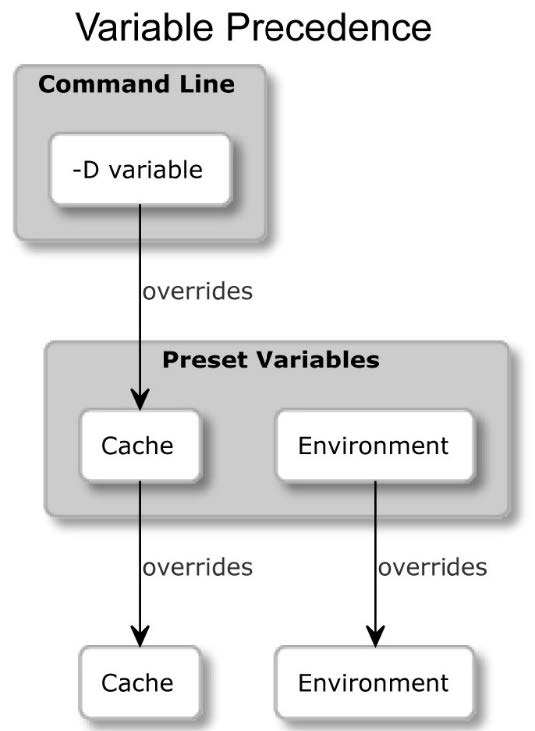
\includegraphics[width=0.5\textwidth]{content/1/chapter1/images/3.jpg}\\
Figure 1.3 – How presets override CMakeCache.txt and the system environment variables
\end{center}

\hspace*{\fill} \\ %插入空行
\noindent
\textbf{Building a project}

After generating our build tree, we're ready for the next stage: running the builder tool. Not only does CMake know how to generate input files for many different builders, but it can also run them for you with arguments that are specific to our project.

\begin{tcolorbox}[colback=blue!5!white,colframe=blue!75!black,title=Not Recommended]
Many online sources recommend running GNU Make directly after the generation stage: make. This is a default generator for Linux and macOS, and it usually works. However, we prefer the method described in this section, as it is generator-independent and is supported across all platforms. As a result, we don't need to worry about the exact environment of every user of our application.
\end{tcolorbox}

\textbf{The syntax of the build mode}

\begin{tcblisting}{commandshell={}}
cmake --build <dir> [<options>] [-- <build-tool-options>]
\end{tcblisting}

In the majority of these cases, it is enough to simply provide the bare minimum to get a successful build:

\begin{tcblisting}{commandshell={}}
cmake --build <dir>
\end{tcblisting}

CMake needs to know where the build tree is that we generated. This is the same path that we passed with the -B argument in the generation stage.

By providing a few options, CMake allows you to specify key build parameters that work for every builder. If you need to provide special arguments to your chosen, native builder, pass them at the end of the command after the -{}- token:

\begin{tcblisting}{commandshell={}}
cmake --build <dir> -- <build-tool-options>
\end{tcblisting}

\hspace*{\fill} \\ %插入空行
\noindent
\textbf{Options for parallel builds}

By default, many build tools will use multiple concurrent processes to leverage modern processors and compile your sources in parallel. Builders know the structure of project  dependencies, so they can simultaneously process steps that have their dependencies met to save users' time.

You might want to override that setting if you're building on a powerful machine (or to force a single-threaded build for debugging). Simply specify the number of jobs with either of the following options:

\begin{tcblisting}{commandshell={}}
cmake --build <dir> --parallel [<number-of-jobs>]
cmake --build <dir> -j [<number-of-jobs>]
\end{tcblisting}

The alternative is to set it with the CMAKE\_BUILD\_PARALLEL\_LEVEL environment variable. As usual, we can always use the preceding option to override the variable.

\hspace*{\fill} \\ %插入空行
\noindent
\textbf{Options for target}

We'll discuss targets in the second part of the book. For now, let's just say that every project is made up of one or more parts, called targets. Usually, we'll want to build all of them; however, on occasion, we might be interested in skipping some or explicitly building a target that was deliberately excluded from normal builds. We can do this as follows:

\begin{tcblisting}{commandshell={}}
cmake --build <dir> --target <target1> -t <target2> ...
\end{tcblisting}

As you will observe, we can specify multiple targets by repeating the -t argument.

One target that isn't normally built is clean. This will remove all artifacts from the build directory. You can call it like this:

\begin{tcblisting}{commandshell={}}
cmake --build <dir> -t clean
\end{tcblisting}

Additionally, CMake offers a convenient alias if you'd like to clean first and then implement a normal build:

\begin{tcblisting}{commandshell={}}
cmake --build <dir> --clean-first
\end{tcblisting}

\hspace*{\fill} \\ %插入空行
\noindent
\textbf{Options for multi-configuration generators}

So, we already know a bit about generators: they come in different shapes and sizes. Some of them offer more features than others, and one of these features is the ability to build both Debug and Release build types in a single build tree.

Generators that support this feature include Ninja Multi-Config, Xcode, and Visual Studio. Every other generator is a single-configuration generator, and they require a separate build tree for that purpose.

Select Debug, Release, MinSizeRel, or RelWithDebInfo and specify it as follows:

\begin{tcblisting}{commandshell={}}
cmake --build <dir> --config <cfg>
\end{tcblisting}

Otherwise, CMake will use Debug as the default.

\hspace*{\fill} \\ %插入空行
\noindent
\textbf{Options for debugging}

When things go bad, the first thing we should do is check the output messages. However, veteran developers know that printing all the details all of the time is confusing, so they often hide them by default. When we need to peek under the hood, we can ask for far more detailed logs by telling CMake to be verbose:

\begin{tcblisting}{commandshell={}}
cmake --build <dir> --verbose
cmake --build <dir> -v
\end{tcblisting}

The same effect can be achieved by setting the CMAKE\_VERBOSE\_MAKEFILE cached variable.

\hspace*{\fill} \\ %插入空行
\noindent
\textbf{Installing a project}

When artifacts are built, users can install them on the system. Usually, this means copying files into the correct directories, installing libraries, or running some custom installation logic from a CMake script.

\textbf{The syntax of the installation mode}

\begin{tcblisting}{commandshell={}}
cmake --install <dir> [<options>]
\end{tcblisting}

As with other modes of operation, CMake requires a path to a generated build tree:

\begin{tcblisting}{commandshell={}}
cmake --install <dir>
\end{tcblisting}

\hspace*{\fill} \\ %插入空行
\noindent
\textbf{Options for multi-configuration generators}

Just like in the build stage, we can specify which build type we want to use for our installation (for more details, please refer to the Building a project section). The available types include Debug, Release, MinSizeRel, and RelWithDebInfo. The signature is as follows:

\begin{tcblisting}{commandshell={}}
cmake --install <dir> --config <cfg>
\end{tcblisting}

\hspace*{\fill} \\ %插入空行
\noindent
\textbf{Options for components}

As a developer, you might choose to split your project into components that can be installed independently. We'll discuss the concept of components in further detail in Chapter 11, Installing and Packaging. For now, let's just assume they represent different parts of the solution. This might be something like application, docs, and extratools.

To install a single component, use the following option:

\begin{tcblisting}{commandshell={}}
cmake --install <dir> --component <comp>
\end{tcblisting}

\hspace*{\fill} \\ %插入空行
\noindent
\textbf{Options for permissions}

If installation is carried on a Unix-like platform, you can specify default permissions for the installed directories, with the following option, using the format of u=rwx,g=rx,o=rx:

\begin{tcblisting}{commandshell={}}
cmake --install <dir>
  --default-directory-permissions <permissions>
\end{tcblisting}

\hspace*{\fill} \\ %插入空行
\noindent
\textbf{Options for the installation directory}

We can prepend the installation path specified in the project configuration with a prefix of our choice (for example, when we have limited write access to some directories). The /usr/local path that is prefixed with /home/user becomes /home/user/usr/local. The signature for this option is as follows:

\begin{tcblisting}{commandshell={}}
cmake --install <dir> --prefix <prefix>
\end{tcblisting}

Note that this won't work on Windows, as paths on this platform usually start with the drive letter.

\hspace*{\fill} \\ %插入空行
\noindent
\textbf{Options for debugging}

Similarly, to the build stage, we can also choose to view a detailed output of the installation stage. To do this, use any of the following:

\begin{tcblisting}{commandshell={}}
cmake --build <dir> --verbose
cmake --build <dir> -v
\end{tcblisting}

The same effect can be achieved if the VERBOSE environment variable is set.

\hspace*{\fill} \\ %插入空行
\noindent
\textbf{Running a script}
 
CMake projects are configured using CMake's custom language. It's cross-platform, quite powerful, and already present. So, why not make it available for other tasks? Sure enough, you can write standalone scripts (we'll get to that at the end of this chapter).

CMake can run these scripts like so:

\textbf{Syntax of the script mode}

\begin{tcblisting}{commandshell={}}
cmake [{-D <var>=<value>}...] -P <cmake-script-file>
      [-- <unparsed-options>...]
\end{tcblisting}

Running such a script won't run any configurations or generate stages. Additionally, it won't affect the cache. There are two ways you can pass values to this script:

\begin{itemize}
\item 
Through variables defined with the -D option.

\item 
Through arguments that can be passed after a -{}- token. CMake will create CMAKE\_ARGV<n> variables for all arguments passed to the script (including the -{}- token).
\end{itemize}

\hspace*{\fill} \\ %插入空行
\noindent
\textbf{Running a command-line tool}

On rare occasions, we might need to run a single command in a platform-independent way – perhaps copy a file or compute a checksum. Not all platforms were created equal, so not all commands are available in every system, or they have a different name.

CMake offers a mode in which to execute the most common ones in the same way across platforms:

\textbf{The syntax of the command-line tool mode}

\begin{tcblisting}{commandshell={}}
cmake -E <command> [<options>]
\end{tcblisting}

As the use of this particular mode is fairly limited, we won't cover it in depth. However, if you're interested in the details, I recommend calling cmake -E to list all the available commands. To simply get a glimpse of what's on offer, CMake 3.20 supports the following commands:

capabilities, cat, chdir, compare\_files, copy, copy\_directory, copy\_if\_different, echo, echo\_append, env, environment, make\_directory, md5sum, sha1sum, sha224sum, sha256sum, sha384sum, sha512sum, remove, remove\_directory, rename, rm, server, sleep, tar, time, touch, touch\_nocreate, create\_symlink, create\_hardlink, true, and false.
 
If a command you'd like to use is missing, or you need a more complex behavior, consider wrapping it in a script and running it in -P mode.

\hspace*{\fill} \\ %插入空行
\noindent
\textbf{Getting help}

It comes without surprise that CMake offers extensive help that is accessible through its command line.

\textbf{The syntax of the help mode}

\begin{tcblisting}{commandshell={}}
cmake ––help[-<topic>]
\end{tcblisting}

\subsubsubsection{1.4.2\hspace{0.2cm}CTest}

Automated testing is very important in order to produce and maintain high-quality code. That's why we devoted an entire chapter to this subject (please refer to Chapter 8, Testing Frameworks), where we do a deep dive into the usage of CTest. It is one of the available command-line tools, so let's briefly introduce it now.

CTest is about wrapping CMake in a higher layer of abstraction, where the building stage becomes just one of the stepping stones in the process of developing our software. Other tasks that CMake can do for us include updating, running all kinds of tests, reporting the state of the project to external dashboards, and running scripts written in the CMake language.

More importantly, CTest standardizes running tests and reporting for solutions built with CMake. This means that as a user, you don't need to know which testing framework the project is using or how to run it. CTest provides a convenient façade to list, filter, shuffle, retry, and timebox test runs. Additionally, it can call CMake for you if a build is required.

The simplest way to run tests for a built project is to call ctest in the generated build tree:

\begin{tcblisting}{commandshell={}}
$ ctest
Test project C:/Users/rapha/Desktop/CMake/build
Guessing configuration Debug
    Start 1: SystemInformationNew
1/1 Test #1: SystemInformationNew ......... Passed 3.19 sec

100% tests passed, 0 tests failed out of 1
Total Test time (real) = 3.24 sec
\end{tcblisting}

\subsubsubsection{1.4.3\hspace{0.2cm}CPack}

After we have built and tested our amazing software, we are ready to share it with the world. In a rare few instances, power users are completely fine with the source code, and that's what they want. However, the vast majority of the world is using precompiled binaries because of convenience and to save time.

CMake doesn't leave you stranded here; it comes with batteries included. CPack is built for the exact purpose of creating packages for different platforms: compressed archives, executable installers, wizards, NuGet packages, macOS bundles, DMG packages, RPMs, and more.

CPack works in a very similar way to CMake: it is configured with the CMake language and has many package generators to pick from (just don't confuse them with CMake buildsystem generators). We'll go through all the specific details in Chapter 11, Installing and Packaging, as this is quite a hefty tool that is meant for the final stages of CMake projects.

\subsubsubsection{1.4.4\hspace{0.2cm}The CMake GUI}

CMake for Windows comes with a GUI version to configure the building process of previously prepared projects. For Unix-like platforms, there is a version built with QT libraries. Ubuntu offers it in the cmake-qt-gui package.

To access the CMake GUI, run the cmake-gui executable:

\begin{center}
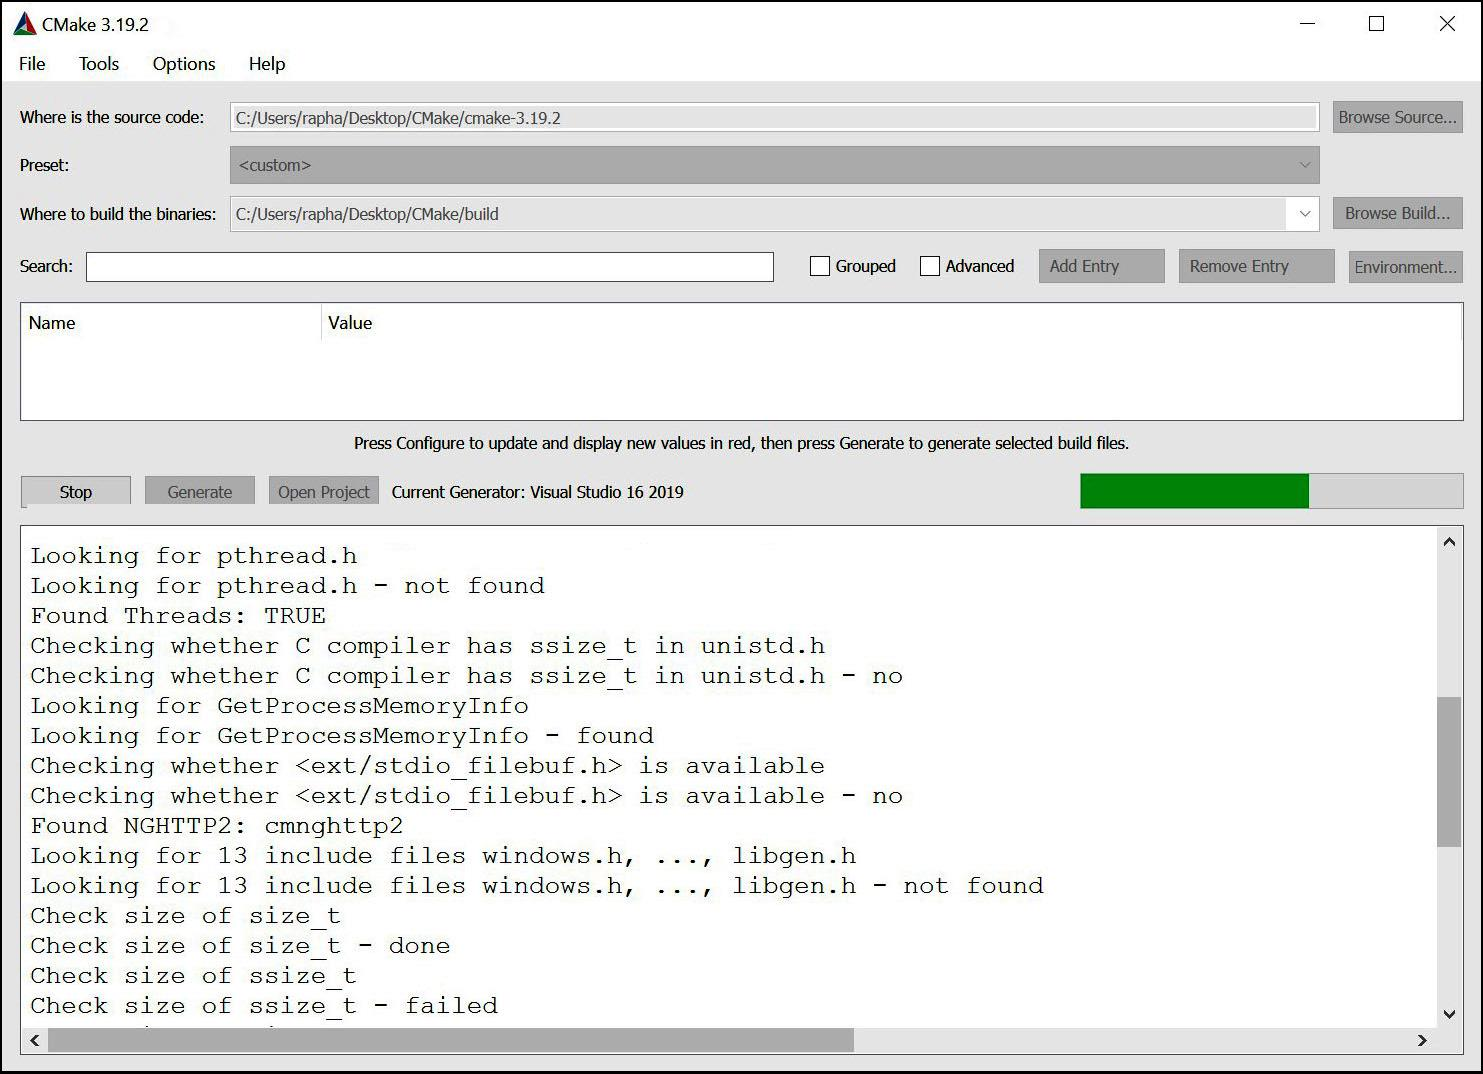
\includegraphics[width=0.9\textwidth]{content/1/chapter1/images/4.jpg}\\
Figure 1.4 – The CMake GUI – the configuring stage for a buildsystem using a generator for Visual Studio 2019
\end{center}

The GUI application is a convenient tool for users of your application, as the options found there are rather limited. It can be useful for those who aren't familiar with the command line and would prefer a window-based interface.

\begin{tcolorbox}[colback=blue!5!white,colframe=blue!75!black,title=Not Recommended]
I would definitely recommend GUI to end users craving convenience; however, as a programmer, I avoid introducing any manual, blocking steps that would require clicking on forms every time I build my programs. This is especially important for build automation in CI pipelines. These tools require headless applications so that the build can be fully executed without any user interaction.
\end{tcolorbox}

\subsubsubsection{1.4.5\hspace{0.2cm}CCMake}

The ccmake executable is the CMake curses interface for Unix-like platforms (it's  unavailable for Windows). It's not available as part of the CMake package, so users have to  install it separately.
 
The command for Debian/Ubuntu systems is as follows:
 
\begin{tcblisting}{commandshell={}}
$ sudo apt-get install cmake-curses-gui
\end{tcblisting}
 
Note that the project configuration settings can be specified interactively through this GUI. Brief instructions are provided at the bottom of the Terminal when the program is running: 

\textbf{The syntax of the CCMake command}
 
\begin{tcblisting}{commandshell={}}
ccmake [<options>]
ccmake {<path-to-source> | <path-to-existing-build>}
\end{tcblisting}
 
CCMake uses the same set of options as cmake:
 
\begin{center}
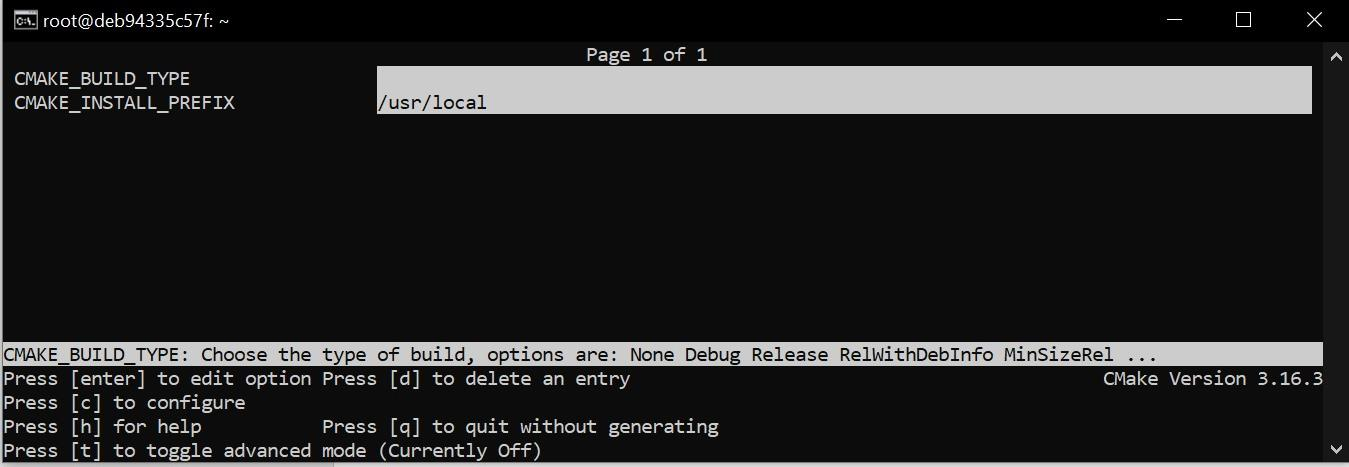
\includegraphics[width=0.9\textwidth]{content/1/chapter1/images/5.jpg}\\
Figure 1.5 – The configuring stage in ccmake
\end{center}
 
As with Graphical User Interfaces (GUIs), this mode is fairly limited and is intended to be used by less experienced users. If you're using a Unix machine, I recommend that you take a quick look and move on even quicker.

This concludes the basic introduction to command line of CMake. It's time to discover what is the structure of a typical CMake project.
 
 
 
 
 
 
 
 
 
 
 
 
 
 
 
 